%% ------------------------------------------------------------------------- %%
\chapter{Introdução}
\label{cap:introducao}

Desenvolvimento Guiado pelos Testes (DGT), em uma tradução do termo
em inglês \textit{Test-Driven Development},
é uma das práticas dentre as sugeridas na Programação
Extrema (XP) \cite{XPExplained}. É baseada em um pequeno ciclo de
desenvolvimento, no qual o desenvolvedor deve sempre escrever um teste antes
de implementar a funcionalidade esperada, e depois, com o código
passando no recém-criado teste, o desenvolvedor refatora para 
remover duplicação de dados e de código \cite{TDDByExample}.
Apesar da constante escrita de testes automatizados, os benefícios da
prática vão além disso. Na opinião de muitos autores conhecidos como Robert Martin,
Steve Freeman e Dave Astels, DGT promove
uma melhoria significativa no projeto de classes, auxiliando o programador a
criar classes mais coesas e menos acopladas \cite{TDDByExample} \cite{GOOS} 
\cite{astels-tdd}.

Criar classes ou, em um nível maior de abstração, módulos que possuam um baixo
acoplamento e uma alta coesão demandam um esforço muito grande do desenvolvedor. 
É muito comum, após algum tempo de desenvolvimento, que o projeto de classes perca qualidade
e qualquer tipo de manutenção se torne difícil e, por consequência, custosa.
Muitas práticas objetivam reduzir esses problemas, como programação pareada ou
revisão de código. Os praticantes de DGT acreditam que os testes sejam uma outra
maneira de validar o projeto de classes criado, e utilizam esse \textit{feedback} para melhorá-lo.

Em um questionário de 2010 para descobrir quais práticas eram feitas por times
ágeis \cite{wambler-survey-agile}, Scott Ambler mostrou que 53\% dos times ágeis
adotaram DGT como uma maneira para validar o trabalho feito, conforme mostra a 
Figura \ref{fig:wambler-agile-2010}. Outro questionário, de 2008, também realizado por Ambler
\cite{wambler-survey-tdd}, focado em DGT, mostra que 57\% dos desenvolvedores 
utilizam DGT como técnica para capturar informações de projeto de classes, conforme mostrado
na Figura \ref{fig:wambler-tdd-2008}.

Robert Martin chega a relacionar DGT à responsabilidade de um 
profissional de desenvolvimento de software. 
Segundo ele, DGT favorece que o desenvolvedor entregue um 
código claro, flexível, que funciona, e dentro do prazo \cite{martin-profissionalismo}.
Muitos desenvolvedores que experimentam essa prática raramente voltam atrás e deixam
de escrever os testes antes \cite{tdd-fearless}. 

Uma vez que testes de unidade são intrísecos à prática de DGT, 
grande parte dos experimentos feitos pela academia verificam os
efeitos da prática na qualidade externa. Conforme é discutido no capítulo de
trabalhos relacionados, poucos são os estudos que avaliam DGT do
ponto de vista da qualidade interna do código, e muitos desses estudos
são feitos somente com estudantes, diminuindo o realismo do experimento. 
Siniaalto e Abrahamsson \cite{alarming-results} também
compartilham dessa opinião e, além disso, notaram que os efeitos de DGT podem 
não ser tão automáticos ou evidentes como o esperado.

Apesar da pouca quantidade, alguns experimentos mostram que DGT tem uma influência
positiva no projeto de classes, diminuindo o grau de acoplamento, aumentando
a coesão e a simplicidade de suas classes e módulos. Entretanto, poucos trabalhos
levam em consideração a experiência do desenvolvedor e diversos
outros fatores que podem influenciar na qualidade final do código, como conhecimento
de príncipios de orientação a objetos ou experiência com o processo de 
desenvolvimento de software. Além disso, poucos trabalhos também discutem como
a prática de DGT realmente influencia 
nas decisões de projeto de classes tomadas pelos desenvolvedores durante a criação de sistemas 
orientados a objetos.

Avaliar os efeitos de DGT no projeto de classes é difícil, mas extremamente importante.
Ao entender melhor como efetivamente a prática guia o desenvolvedor durante
a criação do projeto de classes, desenvolvedores podem maximizar esse \textit{feedback},
e tirar maior proveito do que a prática tende a oferecer. Ao perceber 
problemas de projeto de classes mais cedo e, por consequência, resolvê-los
mais cedo, programadores diminuem o custo de manutenção evolutiva dos projetos
de software que, geralmente tendem a ser elevados.

Conduzir uma pesquisa no mundo real implica um equilíbrio entre o nível de controle
e o grau de realismo. Uma situação realística é, geralmente, complexa e 
não determinística, dificultando o entendimento sobre o que acontece. Por outro
lado, aumentar o controle sobre o experimento reduz o grau de realismo, muitas
vezes fazendo com que os reais fatores de influência fiquem fora do escopo do 
estudo \cite{guidelines-case-study}.
Baseando-se no fato de que o processo de desenvolvimento de software envolve 
diversos fatores humanos e é totalmente sensível ao contexto em que ele está 
inserido, 
este estudo faz uso de uma combinação entre um experimento controlado inicial, 
no qual participantes serão convidados a resolver exercícios utilizando DGT e, 
a partir dos dados colhidos nesse estudo, um outro estudo qualitativo entrará em 
detalhes objetivando entender como a prática influenciou as decisões de projeto 
dos participantes. Os métodos de pesquisa utilizados por
esse trabalho são apresentados no Capítulo \ref{cap:planejamento}.

\begin{figure}[ht]
  \begin{minipage}[b]{0.45\linewidth}
    \centering
    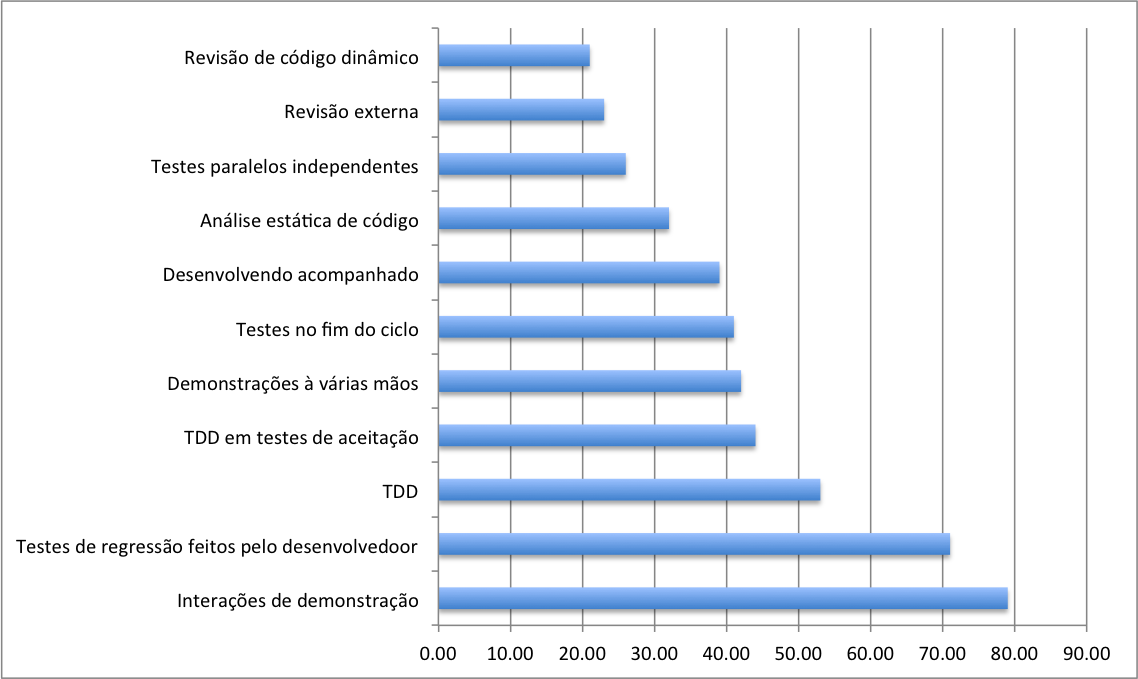
\includegraphics[scale=.4]{agileCriteria2010Validating-pt}
    \caption{Como times ágeis validam seu próprio trabalho?}
    \label{fig:wambler-agile-2010}
  \end{minipage}
  \hspace{0.5cm}
  \begin{minipage}[b]{0.45\linewidth}
    \centering
    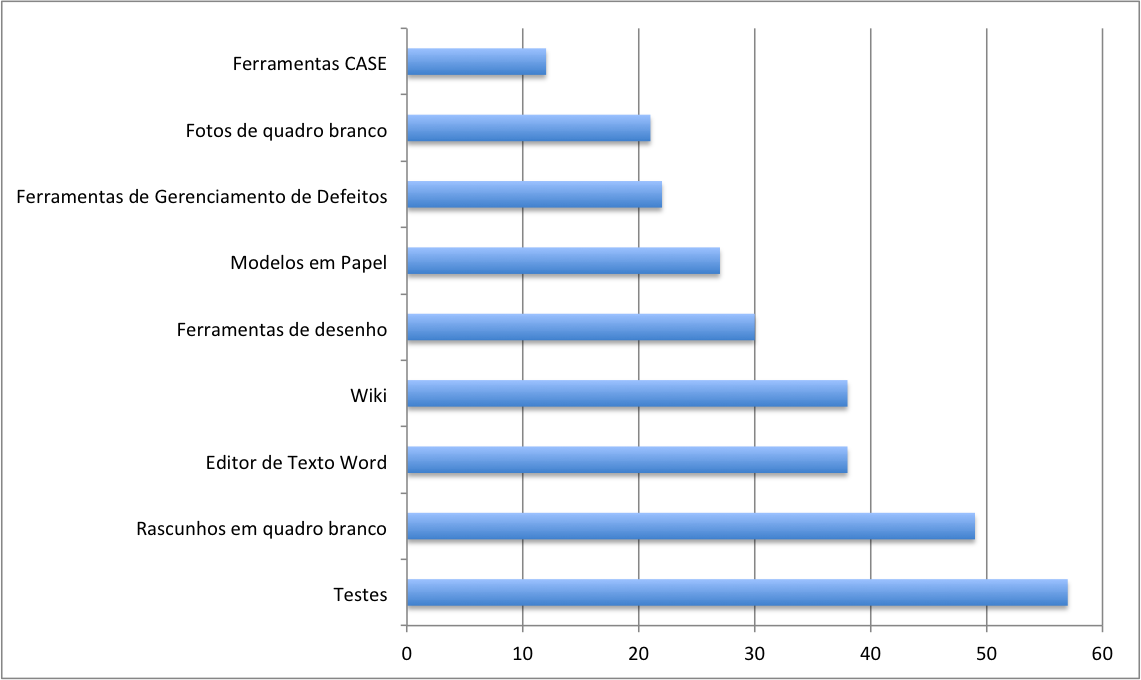
\includegraphics[scale=.4]{tddDesignPractices-pt}
    \caption{Práticas que desenvolvedores ágeis usam para auxiliar no projeto de classes}  
    \label{fig:wambler-tdd-2008}
  \end{minipage}
\end{figure}			

%% ------------------------------------------------------------------------- %%
\section{Motivação}

Esta pesquisa possui diversas motivações. A primeira delas é a crescente
popularidade da prática de DGT, tanto por parte da indústria, quanto 
por parte da academia. O número de desenvolvedores, experientes e inexperientes,
que aplicam DGT cresce cada vez mais, e isso pode ser empiricamente
observado através do número de participantes em palestras de DGT nos
eventos de desenvolvimento de software brasileiros, vagas de emprego
que pedem que o desenvolvedor conheça a prática, e etc.

No entanto, conforme discutido no estudo que fizemos 
realizado em 2010 dentro de uma conferência de 
métodos ágeis, e publicado no WBMA 2010 \cite{aniche-wbma}, apesar da prática de 
DGT ter crescido em popularidade, os desenvolvedores não souberam
colocar em palavras quais eram os efeitos da prática no projeto de classes.
Isso nos leva a crer que os deenvolvedores ainda 
não compreendem muito bem estes efeitos.

É de extrema importância conhecer os reais efeitos de DGT no projeto de classes. Com essa
informação em mãos, desenvolvedores podem aproveitar ao máximo
a prática e melhorar ainda mais a qualidade dos seus projetos
de classe. 
Este trabalho, além de poder explicar ao desenvolvedor os efeitos
da prática, ainda pode servir de apoio à decisão da adoção da prática
de DGT nos times de desenvolvimento.

%% ------------------------------------------------------------------------- %%
\section{Contribuições}

Este trabalho
visa compreender a real influencia de DGT no projeto de classes.
Mais profundamente, este trabalho avalia a relação entre a prática de 
DGT
e as decisões de projeto de classes tomadas pelos desenvolvedores no processo de 
criação de classes.

A análise será feita por meio de dados que serão
capturados baseados na percepção de programadores atuantes na indústria, após
a implementação de alguns pequenos problemas especialmente criados para
esta pesquisa.

O objetivo principal deste estudo é \textbf{entender a relação da prática de DGT 
e as decisões de projeto de classes tomadas pelo programador durante o processo de 
projeto de sistemas orientados a objetos}.
Para compreendê-la, tenta-se responder às questões listadas
abaixo:

\begin{enumerate}

	\item Qual a influência de DGT no projeto de classes?

	\item Qual a relação entre DGT e as tomadas de decisões de projeto
	feitas por um desenvolvedor?

	\item Como a prática de DGT influencia o programador no processo de  
	projeto de classes, do ponto de vista do acoplamento, coesão e complexidade?

\end{enumerate}

%% ------------------------------------------------------------------------- %%
\section{Organização do trabalho}

Este trabalho está dividido da seguinte maneira: 

\begin{itemize}
	\item O Capítulo \ref{cap:tdd} discute sobre a prática de DGT, com ênfase no
	ponto de vista do projeto de classes;
  
	\item O Capítulo \ref{cap:trabalhos-relacionados} mostra trabalhos já
	realizados pela academia sobre os efeitos de DGT;

	\item O Capítulo \ref{cap:planejamento} discute o planejamento do experimento,
	bem como o processo de captura de dados e análise;

	\item O Capítulo \ref{cap:discussao} apresenta os resultados encontrados e
	os discute;
	
	\item O Capítulo \ref{cap:ameacas} discute as possíveis ameaças aos resultados
	encontrados na pesquisa;
	
	\item O Capítulo \ref{cap:conclusoes} resume o trabalho realizado e apresenta
	possibilidades de trabalhos futuros.
\end{itemize}

